
%=================================================================================================
\section{Introduction}
\label{sec:introduction}

A worldwide effort to directly detect gravitational radiation with large scale laser interferometers 
has been underway for the past several decades.  
In the United States the Laser Interferometer Gravitational-Wave Observatories (LIGO) have been operating
since the early 2000's.  
During this time of operation a significant amount of effort was invested by the LIGO Scientific Collaboration 
to research, design, and build upgrades to the initial LIGO interferometers.  
As of 2011 the initial LIGO detectors were decommissioned and installation of these upgrades began.  
As installation has progressed the integration and commissioning phase has begun for many of the 
upgraded subsystems at the LIGO observatories.  

One of the subsystems undergoing a significant upgrade for the Advanced LIGO era is 
the input optics.  
It is the task of the input optics to clean and stabilize the laser beam from the 
Pre-Stabilized Laser (PSL) before injection into the main interferometer.  
The upgraded sensitivity of the Advanced LIGO interferometers places stringent requirements on 
the stability of the input light and therefore on the input optics.  
In particular, the input optics must supply multiple low amplitude and phase noise RF sidebands.  
They must provide a frequency reference stable enough to not spoil the interferometer's 
gravitational wave sensitivity.  
They must provide mode matching and beam pointing actuation into the interferometer.  
Finally, they must provide isolation between the interferometer's reflected light and the 
input optics chain.  

The next section of this paper, section II, will present the design requirements for the input optics and 
briefly explain how these requirements were derived.  
It will also describe some of the other Advanced LIGO subsystems in only as much detail as 
is necessary for an understanding of the input optics.  
Sections III and IV will give an overview description of the out-of-vacuum and in-vacuum 
components respectively.  
Section V will discuss the input mode cleaner which is at the heart of the input optics, 
both in location and form.  
Section VI will describe the Faraday Isolator whose design is highly customized for high power 
operation.  
Finally, sections VII and IIX will close with a description of the overall power throughput of the 
input optics chain and some conclusions.  

%==================================================================================================
\section{Design Requirements}
\label{sec:design_requirements}

The design requirements for the input optics subsystem derive from the designed sensitivity of the 
interferometer.  
Figure \ref{fig:aLIGODesignSensitivity} shows the design sensitivity of the Advanced LIGO interferometers 
together with the measured sensitivity of one of the Initial LIGO interferometers during the sixth 
science run.  
The Advanced LIGO interferometers are designed to be limited by seismic noise below $\sim$10 Hz, 
radiation pressure noise in the 10-50 Hz range, coating thermal noise between 50 Hz and 200 Hz, 
and photon shot noise above 200 Hz.  
The mantra for setting design requirements for the interferometer subsystems is therefore to keep 
the 'technical noise sources' below this limit.  
In fact the subsystem requirements were set by demanding that the technical noise sources be a factor of 
10 below the design sensitivity\cite{ligo_T070236}.  

%^^^^^^^^^^^^^^^^^^^^^^^^^^^^^^^^^^^^^^^^^^^^^^^^^^^^^^^^^^^^^^^^^^^^^^^^^^^^^^^^^^^^^^^^^^^^^^^^^^
\begin{figure}
	\centering
	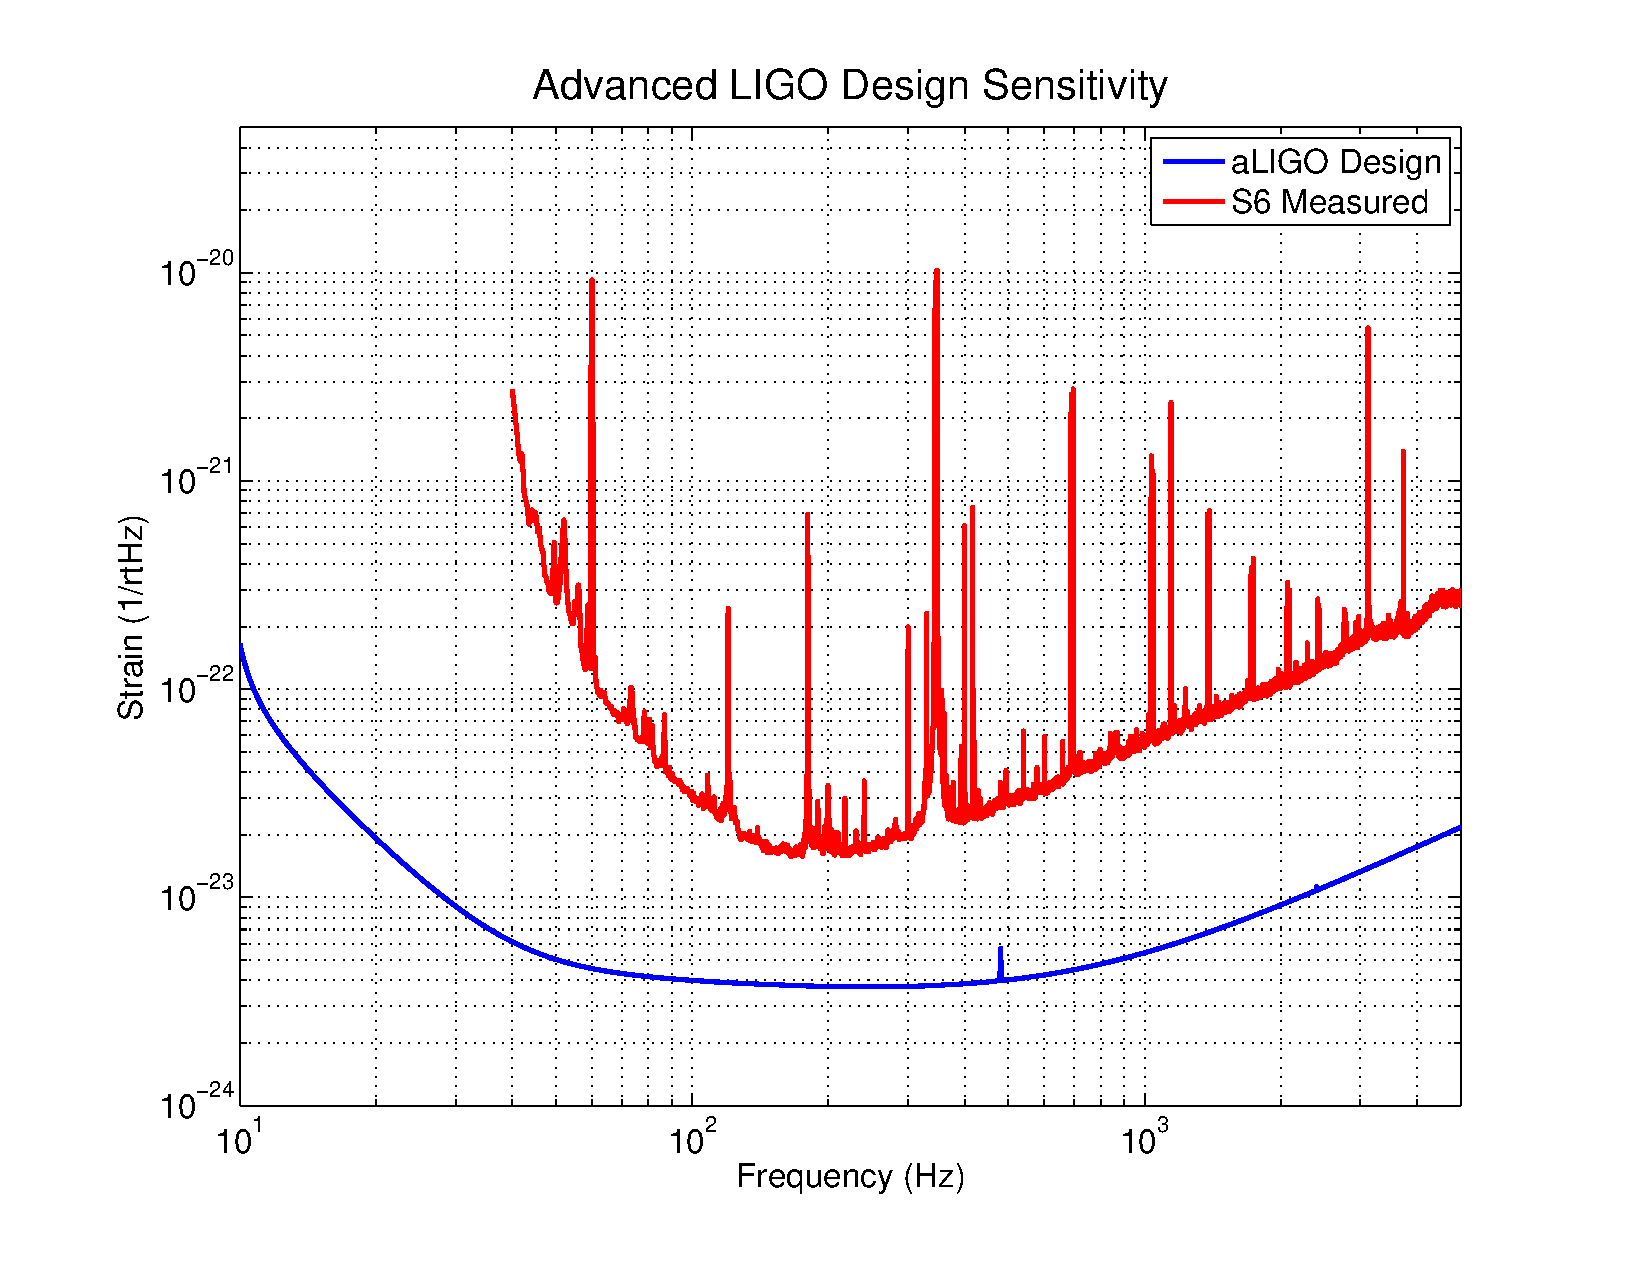
\includegraphics[width = 0.8\textwidth,trim=2cm 1cm 2cm 1cm]{aLIGO_Design_Sensitivity.pdf}
	\caption{The Advanced LIGO design sensitivity\cite{ligo_T0900288} is shown together with the measured 
		sensitivity from the LIGO Hanford Observatory during the sixth LIGO science run\cite{ligo_T1100338}.  
		The design sensitivity includes the fundamental limiting noise sources (quantum, thermal, and seismic) 
		which set the requirements for the interferometer subsystems such as the input optics.}
	\label{fig:aLIGODesignSensitivity}
\end{figure}
%^^^^^^^^^^^^^^^^^^^^^^^^^^^^^^^^^^^^^^^^^^^^^^^^^^^^^^^^^^^^^^^^^^^^^^^^^^^^^^^^^^^^^^^^^^^^^^^^^^

%--------------------------------------------------------------------------------------------------
\subsection{Frequency Noise at the Interferometer Input}
\label{sec:frequency_noise_interferometer}

A perfect Michelson interferometer is completely insensitive to frequency noise; a fact which 
is a large motivator in choosing the Michelson topology for gravitational wave interferometers.  
However any asymmetry between the two arms of the Michelson interferometer will couple frequency 
fluctuations to the output.  
The asymmetries between the two arms depend on many parameters such as: the imbalance between the reflectivity 
and transmissivity of the beam splitter, the reflectivity imbalance of the arm cavity input mirrors, 
different amounts of losses in the two arm cavities, and the static distance asymmetry between the 
beam splitter and the two arm cavities (known as the Schnupp asymmetry).  

Using experience from Initial LIGO and a reasonable estimate of the Advanced LIGO parameters, 
the Interferometer Sensing and Control (ISC) group put together a detailed numerical simulation 
of the full Advanced LIGO interferometer \cite{ligo_T070236}.  
With this simulation they derive the frequency noise requirement at the input to the interferometer 
to be roughly the curve labeled 'Frequency Noise Requirements at Interferometer Input' 
in figure \ref{fig:FreqReqs}.
The frequency noise stabilization for the interferometer is not solely the job of the input optics; 
the final stabilization reference is the average length of the two arms.  
Figure \ref{fig:FreqReqs} also shows the frequency noise requirements after suppression by the common 
arm length feedback servo.  
Also shown are the expected length noise of the input mode cleaner as well as the expected frequency 
noise out of the pre-stabilized laser.  

%^^^^^^^^^^^^^^^^^^^^^^^^^^^^^^^^^^^^^^^^^^^^^^^^^^^^^^^^^^^^^^^^^^^^^^^^^^^^^^^^^^^^^^^^^^^^^^^^^^
\begin{figure}
	\centering
	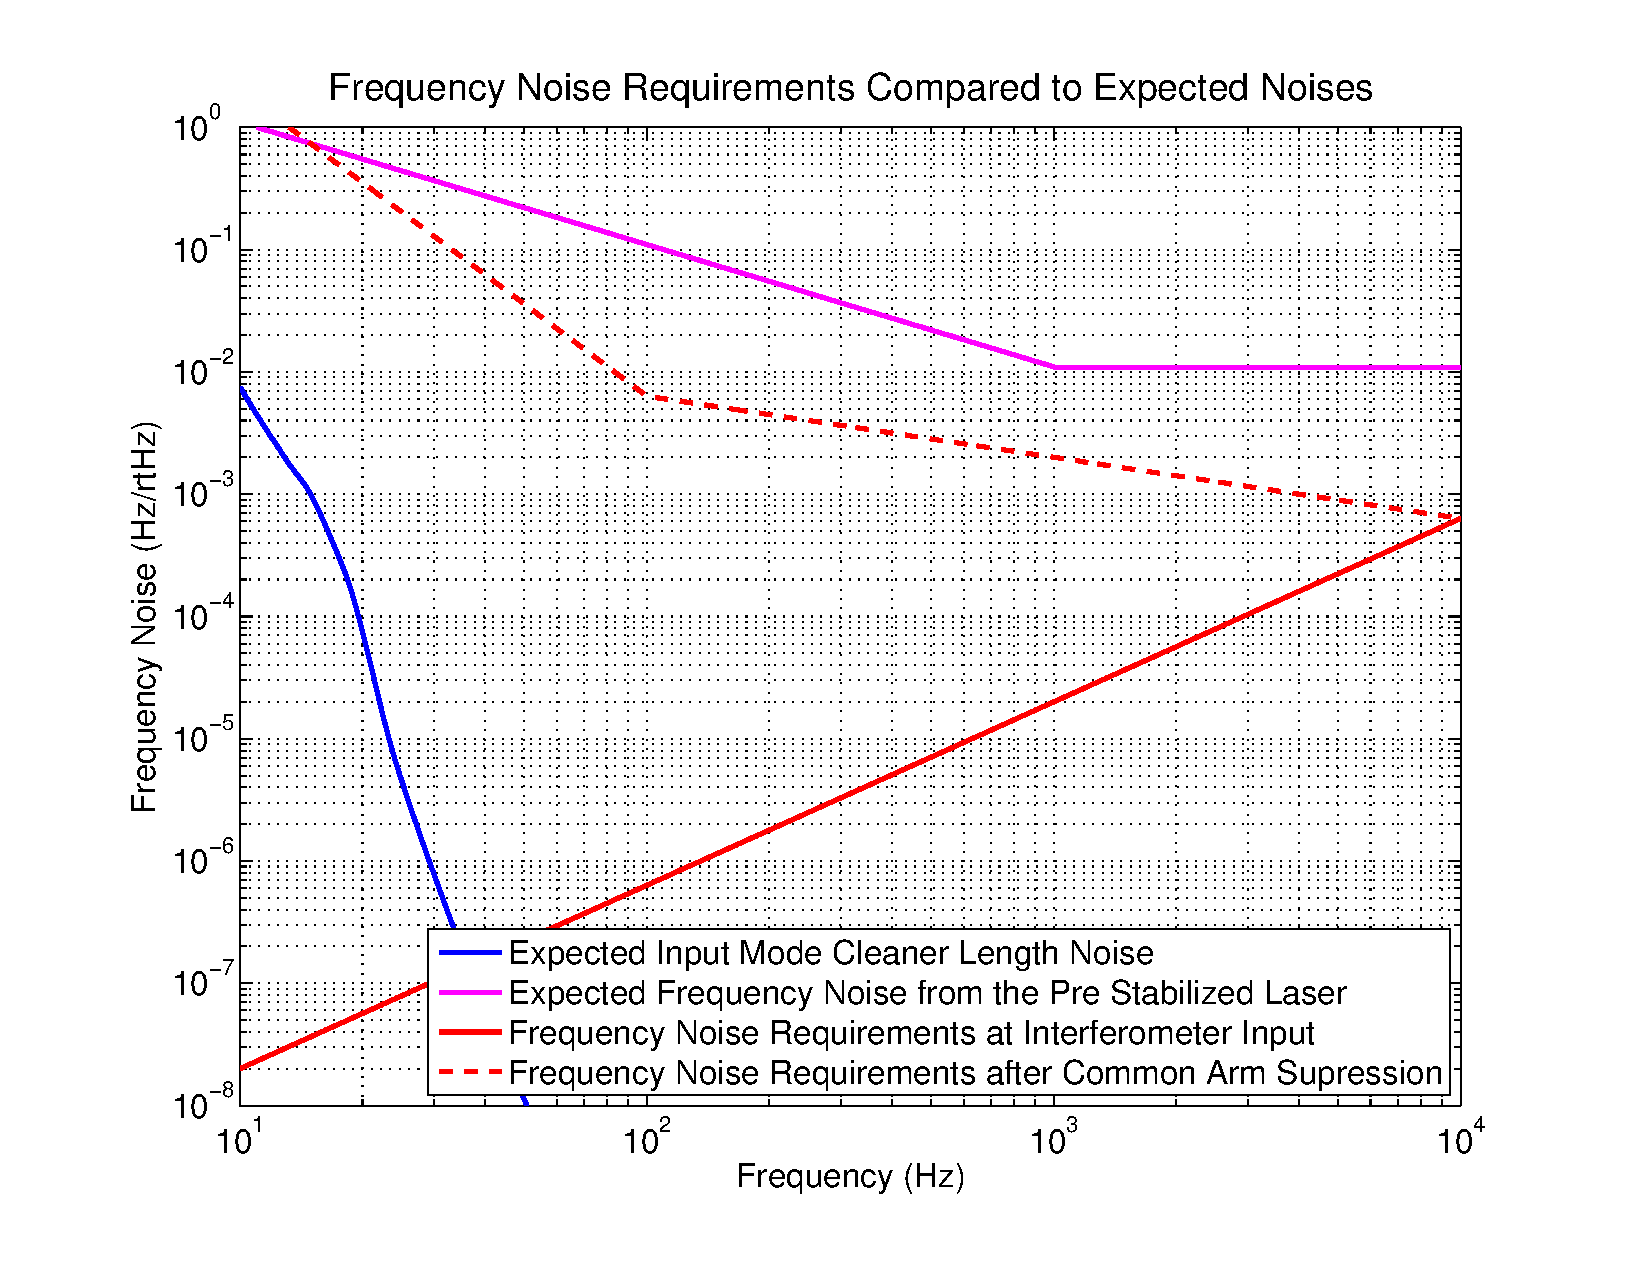
\includegraphics[width = 0.8\textwidth,trim=2cm 1cm 2cm 1cm]{Freq_Noise_Reqs.pdf}
	\caption{The rough frequency noise requirements at the input to the interferometer are shown both 
		with and without the common arm loop suppression.  
		Also shown are the expected length noise of the input mode cleaner and the expected frequency 
		noise out of the pre-stabilized laser (PSL).  
		Ostensibly the job of the input optics is to suppress the frequency noise out of the PSL to 
		the requirements level after the common arm gain is taken into account.  
		In reality acoustic effects in the injection optics between the PSL and the in-vacuum input 
		optics will require a higher level of suppression.}
	\label{fig:FreqReqs}
\end{figure}
%^^^^^^^^^^^^^^^^^^^^^^^^^^^^^^^^^^^^^^^^^^^^^^^^^^^^^^^^^^^^^^^^^^^^^^^^^^^^^^^^^^^^^^^^^^^^^^^^^^

The job of the input optics is therefore to stabilize the laser frequency by roughly a factor of 20 
between 10 Hz and 10 kHz.  
In reality the frequency noise suppression necessary for the input optics is higher because 
acoustic effects in the injection chain will add frequency noise before the light is injected 
to the isolated in-vacuum optics.  


%--------------------------------------------------------------------------------------------------
\subsection{Beam Alignment Noise at the Interferometer Input}
\label{sec:beam_alignment_noise}

As with frequency noise, a perfect Michelson interferometer is first order insensitive to pointing 
noise.  
There are two types of imperfections which couple pointing noise to the gravitational wave 
readout channel.  
The first considered in \cite{ligo_T020022} is caused by residual misalignments of the core interferometer 
optics causing the misaligned beam to rejoin with the main interferometer mode and show up 
in the gravitational wave channel.  
The second coupling is caused by the beam spot motion on the core interferometer optics 
causing the residual angular motion of the optics to couple to the gravitational wave channel.  
These two effects lead to similar noise requirements at the input to the interferometer which 
a beam stability of $4\cdot10^{-10}\ \frac{rad}{\sqrt{Hz}}$ at 100 Hz and above and decreasing 
(getting less stringent) as $f^2$ below 100 Hz.


%--------------------------------------------------------------------------------------------------
\subsection{RF Sidebands}
\label{sec:rf_sidebands}

Sensing and controlling most of the seven degrees of freedom of the interferometer are done by some 
variant of the Pound Drever Hall technique \cite{drever_laser_1983}.  
This technique uses optical heterodyne detection to sense the phase of the returning light from 
an optical cavity by sensing the phase modulation to amplitude modulation conversion which occurs 
when the cavity is slightly off resonance.  
It depends on having low noise radio frequency sidebands to generate detectable beat notes 
with the carrier light.
It is part of the responsibility of the input optics to add these RF sidebands to the laser beam 
before delivering it to the interferometer.  

In particular the input optics are responsible for adding three RF sidebands, one for controlling 
length of the input mode cleaner and two for controlling the other degrees of freedom of the 
interferometer.  
The phase modulator must be able to produce phase modulation depths up to 0.8, and must 
maintain a residual amplitude modulation level below $1\cdot10^{-4}$ $\frac{AM}{PM}$ ratio.  


%--------------------------------------------------------------------------------------------------
\subsection{In-Vacuum Optical Isolation}
\label{sec:in-vacuum_optical_isolation}

The input optics is also required to provide isolation from the light reflected off of the 
interferometer.  
This is necessary to avoid inadvertently forming an optical cavity between the components 
of the input optics and the rest of the interferometer, 
an effect usually referred to as parasitic interferometry.  
Based on experience with parasitic interferometers in initial LIGO and power scaling arguments 
the isolation requirement level was set at 30 dB\cite{ligo_T020020}.  


%--------------------------------------------------------------------------------------------------
\subsection{Throughput and Availability}
\label{sec:throughput_availability}

The final requirements on the input optics are placed on the amount of light which is delivered 
to the interferometer and the amount of time which the input mode cleaner is available.  
In order to deliver the 125 W of laser power required for full power operation the input optics 
must achieve 75\% throughput at all power levels including static and thermal mode matching losses.  
Additionally, in order not to spoil the detection availability of the interferometer 
it is required that the input mode cleaner re-lock time be less than 20 seconds.  
